%%%%%%%%%%%%%%%%%%%%%%%%%%%%%%%%
% Classe do documento
%%%%%%%%%%%%%%%%%%%%%%%%%%%%%%%%

\documentclass[engenharia]{UnB-CIC}%
\usepackage{pdfpages}% incluir PDFs, usado no apêndice
\usepackage{natbib}
\usepackage{url}  % Para usar URLs no BibTeX
\usepackage{chngcntr}
\usepackage{adjustbox}

\counterwithout{figure}{chapter} % Remove a dependência do capítulo

%%%%%%%%%%%%%%%%%%%%%%%%%%%%%%%%
% Informações do Trabalho
%%%%%%%%%%%%%%%%%%%%%%%%%%%%%%%%
\orientador{\prof \dr Alexandre Ricardo Soares Romariz}{CIC/UnB}%
%\coorientador{\prof \dr José Ralha}{CIC/UnB}
\coordenador{\prof \dr João Luiz Azevedo de Carvalho}{Bibliothèque universelle de Genève}%
\diamesano{12}{agosto}{2024}%

\autor{João Victor Alves dos}{Santos}%

\titulo{MatchPredict AI: Melhorando a Compatibilidade de Relacionamentos em Aplicativos de Namoro}%

\palavraschave{Inteligência Artificial, Relacionamentos Virtuais, Previsão de Sucesso de Relacionamento, trabalho de conclusão de curso}%
\keywords{Artificial Intelligence, Virtual Relationships, Relationship Success Prediction, thesis}%

\newcommand{\unbcic}{\texttt{UnB-CIC}}%

%%%%%%%%%%%%%%%%%%%%%%%%%%%%%%%%
% Texto
%%%%%%%%%%%%%%%%%%%%%%%%%%%%%%%%
\begin{document}%

\section{Introdução}%
    \subsection{Contexto}
Na era digital, os relacionamentos evoluíram significativamente, com a tecnologia desempenhando um papel central na forma como as pessoas se conectam. Aplicativos de namoro como Tinder, Hinge e Coffee Meets Bagel utilizam IA para analisar grandes volumes de dados comportamentais dos usuários, personalizando as sugestões de parceiros de forma a aumentar as chances de matches bem-sucedidos.

A relevância da IA nesses aplicativos está na sua capacidade de identificar padrões de comportamento e prever compatibilidade entre os usuários. Por exemplo, algoritmos de recomendação, semelhantes aos utilizados por plataformas de streaming como Netflix, são aplicados para oferecer sugestões personalizadas com base no histórico de interações e preferências dos usuários. Essa personalização melhora a experiência do usuário, proporcionando recomendações mais precisas e relevantes \textcolor{blue}{[\cite{Bonilla2023}]}.

Estudos recentes mostram que a IA não apenas sugere parceiros, mas também pode prever a estabilidade e a longevidade dos relacionamentos. Análises de dados comportamentais, como frequência de comunicação e interesses comuns, são fatores que contribuem para a previsão da viabilidade dos relacionamentos. Aplicativos como Blush e Aimm utilizam testes de personalidade e análise de preferências físicas para treinar seus sistemas de IA, prometendo maiores chances de encontrar uma combinação perfeita \textcolor{blue}{[\cite{Finkel2012}]}.

Os benefícios da aplicação de IA em aplicativos de namoro incluem a capacidade de fornecer recomendações mais precisas e personalizadas, aumentando as chances de formar relacionamentos significativos. Além disso, a eficiência das conexões melhora, facilitando encontros mais rápidos e criativos. No entanto, existem desafios importantes, como a proteção da privacidade dos dados dos usuários e a necessidade de evitar vieses nos algoritmos, que podem afetar a equidade nas recomendações \textcolor{blue}{[\cite{Sharabi2022}]}.

Aplicativos como Tinder utilizam IA para analisar interações e preferências dos usuários, ajustando-se dinamicamente ao comportamento do usuário ao longo do tempo. Coffee Meets Bagel foca em conexões através de amigos em comum, utilizando dados de redes sociais para criar um senso de confiança e familiaridade entre os usuários, promovendo interações mais significativas \textcolor{blue}{[\cite{Saban2024}]}.

A aplicação de IA em aplicativos de namoro representa uma área promissora, oferecendo soluções inovadoras para melhorar a eficácia dos relacionamentos virtuais. Contudo, é essencial abordar os desafios éticos e técnicos para garantir que essas tecnologias beneficiem os usuários de maneira justa e segura. A privacidade dos dados, a transparência nos algoritmos e a atualização constante das tecnologias são aspectos cruciais para o sucesso e a aceitação dessas ferramentas.

Ao investigar a aplicação de IA em aplicativos de namoro, este estudo contribui para o entendimento das interações virtuais e oferece insights valiosos para o desenvolvimento de estratégias mais eficazes em plataformas de namoro online. A análise criteriosa de dados e algoritmos atuais visa fornecer uma base sólida para futuras pesquisas e inovações na área. A possibilidade de integrar variáveis psicológicas e sociológicas mais complexas representa uma direção futura promissora para aprimorar ainda mais a precisão e a eficácia dos algoritmos de recomendação.
\subsection{Objetivo}
O presente trabalho de conclusão de curso (TCC) tem como objetivo central explorar e implementar metodologias de inteligência artificial (IA) em um contexto de aplicativo de namoro, com a finalidade de desenvolver um algoritmo de matchmaking mais completo. Este algoritmo não se limitará apenas à recomendação de usuários, mas também à previsão de potenciais usuários para um relacionamento de sucesso e estável. A implementação deste algoritmo será realizada em um contexto real, em um aplicativo de namoro funcional.

\subsection*{Justificativa do Objetivo}

\begin{enumerate}
    \item \textbf{Transformação dos Algoritmos de Matchmaking}\\
    Tradicionalmente, os algoritmos de matchmaking em aplicativos de namoro se baseiam em dados demográficos básicos e preferências superficiais. No entanto, a introdução de IA permite uma análise mais profunda e personalizada das preferências dos usuários. Algoritmos de IA, como o "Most Compatible" do Hinge, utilizam aprendizado de máquina para analisar as preferências e ações dos usuários, sugerindo matches altamente compatíveis. Esta abordagem tem demonstrado aumentar significativamente as chances de matches bem-sucedidos, promovendo conexões mais significativas e duradouras.

    \item \textbf{Previsão de Relacionamentos Estáveis}\\
    A aplicação de IA para prever a estabilidade de relacionamentos vai além da simples correspondência de perfis. Estudos mostram que algoritmos podem ser desenvolvidos para analisar aspectos mais profundos, como comportamentos e interações dos usuários, facilitando previsões sobre a durabilidade e sucesso de um relacionamento. Este avanço é crucial para a evolução dos aplicativos de namoro, proporcionando aos usuários não apenas um parceiro potencial, mas um parceiro com alta probabilidade de um relacionamento duradouro e satisfatório.

    \item \textbf{Implementação em um Contexto Real}\\
    Para validar a eficácia do algoritmo desenvolvido, é essencial sua implementação em um ambiente real. Aplicativos como Tinder e Bumble já utilizam IA para melhorar a experiência do usuário, otimizando fotos de perfil e moderando conteúdo para aumentar a segurança. A implementação em um aplicativo funcional permitirá testar e ajustar o algoritmo em tempo real, garantindo sua eficácia e eficiência no mundo real. Além disso, aplicativos como o Match.com utilizam chatbots com IA para sugerir locais de encontro, mostrando o potencial da IA em oferecer uma experiência de usuário mais completa e personalizada.
\end{enumerate}
\subsection{Organização da Monografia}
\begin{enumerate}
    \item \textbf{Capítulo 2: Padrões Comportamentais}
    \begin{enumerate}
        \item \textbf{Introdução}
        
        Essa seção tem o dever de introduzir os padrões comportamentais mais relevantes para um relacionamento de sucesso. Serão analisados estudos científicos e, além disso, serão investigados padrões comportamentais que são considerados vantajosos e utilizados em aplicativos de relacionamento existentes.

        \item \textbf{Interesses em Comum}
        
        Esta seção irá explorar a influência da personalidade nos relacionamentos. Será discutido como características pessoais, traços psicológicos e interesses em comum podem ser usados para prever a compatibilidade entre usuários. A análise incluirá a revisão de modelos teóricos e estudos empíricos que demonstram a importância da personalidade para a formação de relações duradouras.

        \item \textbf{Conhecidos em Comum (Grafo de Rede Social)}
        
        Nesta parte, a análise se concentrará em como as conexões sociais afetam a probabilidade de sucesso em aplicativos de namoro. Utilizando o conceito de grafos de redes sociais, será discutido o impacto de conhecidos em comum na facilitação de encontros mais confiáveis e com maior potencial de sucesso. Estudos de caso e pesquisas acadêmicas que analisam essa dinâmica serão apresentados.

        \item \textbf{Preferência Visual}
        
        O objetivo desta seção é examinar o papel das preferências visuais no processo de formação de relacionamentos. Será avaliado como os algoritmos podem ser treinados para reconhecer padrões visuais que indicam preferências estéticas e como essas preferências influenciam a atração e a decisão de iniciar um contato.
    \end{enumerate}

    \item \textbf{Capítulo 3: Fundamentação Teórica}
    \begin{enumerate}
        \item \textbf{Convolutional Neural Networks (CNNs)}
        
        Explora o uso de CNNs para extrair características visuais de perfis, melhorando a recomendação de parceiros ao identificar preferências visuais através de imagens.

        \item \textbf{Transformers}
        
        Discute como Transformers utilizam autoatenção para analisar descrições de perfis e mensagens, capturando interesses e compatibilidades em dados sequenciais.

        \item \textbf{Graph Neural Networks (GNNs)}
        
        Aborda como GNNs modelam conexões sociais, propagando informações entre nós para identificar padrões de interação e fortalecer recomendações.

        
    \end{enumerate}
    
    \item \textbf{Capítulo 4: Trabalhos Relacionados}
    \begin{enumerate}
        \item \textbf{Cafe: Predicting Physical Attraction with Deep Learning-Based Systems}
        
        Descreve como o projeto "Cafe" utiliza aprendizado profundo para prever a atratividade física, aplicando CNNs para analisar imagens de perfis em plataformas de namoro.

        \item \textbf{Dataset OkCupid e Instagram Graph API}
        
        Examina como o dataset OkCupid e a API do Instagram Graph podem ser utilizados para aprimorar sistemas de recomendação, focando em agregação de personalidade e social.
        \item \textbf{Graph Neural Networks for Social Recommendation (GraphRecWWW19) and Adaptation}
        
        Analisa o GraphRec, combinando GNNs e atenção para integrar dados de grafos sociais e de itens, com adaptações para incluir traços de personalidade e características visuais.
    \end{enumerate}

    \item \textbf{Capítulo 5: Situação Atual}
    \begin{enumerate}
        \item \textbf{Progresso Atual}
        
        Aqui será apresentado um resumo das atividades realizadas, com ênfase nos resultados obtidos até o momento. Serão destacadas as etapas concluídas e as descobertas mais significativas do projeto.

        \item \textbf{Próximos Passos}
        
        Será identificada e discutida a sequência de etapas futuras necessárias para a conclusão do projeto. Esta seção destacará as prioridades e planos para finalizar o desenvolvimento do algoritmo e sua implementação.

        \item \textbf{Conclusão}
        
        Finalmente, as considerações finais refletirão sobre o trabalho realizado, discutindo as implicações dos resultados para o campo de estudo e propondo direções para pesquisas futuras. A seção também abordará as contribuições do projeto para o avanço dos aplicativos de namoro e suas aplicações práticas.
    \end{enumerate}
\end{enumerate}
%

\section{Introdução}
Este capítulo tratará dos conceitos teóricos essenciais para a elaboração deste Trabalho de Conclusão de Curso, que busca explorar algoritmos de matchmaking em aplicativos de namoro. Inicialmente, serão discutidos os interesses em comum (2.2), que incluem gostos, valores e atividades compartilhadas entre indivíduos, demonstrando como essas semelhanças influenciam a formação e a durabilidade dos relacionamentos.

Em seguida, o capítulo abordará o conceito de conhecidos em comum (2.3), uma estratégia que explora a rede social dos usuários para identificar conexões mútuas que possam facilitar interações e criar um ambiente de confiança entre os possíveis parceiros. Estudos demonstram que conhecidos em comum podem atuar como uma ponte de confiança, aumentando as chances de interação inicial.

Por fim, capítulo também explorará a preferência visual (2.4), analisando como a atratividade física e as primeiras impressões impactam a decisão dos usuários de prosseguir com uma conexão potencial. A compreensão dos padrões visuais preferidos e sua incorporação em algoritmos é fundamental para aprimorar a experiência dos usuários e aumentar a eficácia dos matches sugeridos.


\section{Importância de Interesses e Hobbies Comuns}
\subsection{Efeito de Similaridade-Atração}
O efeito de similaridade-atração é um fenômeno amplamente estudado na psicologia social que sugere que as pessoas são mais propensas a se sentir atraídas por indivíduos que compartilham características semelhantes, como atitudes, interesses e valores. Essa teoria se fundamenta na ideia de que a similaridade proporciona uma base de entendimento mútuo e validação social, elementos cruciais para o desenvolvimento e manutenção de relações interpessoais bem-sucedidas \textcolor{blue}{[\cite{Berscheid1998}]}.

Os estudos sobre o efeito de similaridade-atração indicam que a semelhança entre indivíduos facilita interações mais agradáveis e reforça a percepção de aceitação e pertencimento. Isso ocorre porque os indivíduos são mais propensos a esperar rejeição por parte de pessoas que são dissimilares, enquanto a interação com semelhantes tende a ser mais confortável e agradável Além disso, a similaridade aumenta a probabilidade de encontros casuais em ambientes sociais comuns, como eventos esportivos ou atividades culturais, onde interesses compartilhados são evidentes \textcolor{blue}{[\cite{Newcomb1961}]}.

Outra explicação para o efeito de similaridade-atração é o reforço social, onde interações com indivíduos semelhantes são mais gratificantes, pois reforçam as próprias crenças e atitudes de cada indivíduo. Esse reforço ocorre tanto em contextos de amizade quanto em relacionamentos românticos, onde a validação mútua fortalece o vínculo \textcolor{blue}{[\cite{Byrne1971}]}. Além disso, pesquisas demonstram que, em plataformas de namoro online, perfis que exibem maior similaridade percebida tendem a receber mais interações positivas.

Por fim, é importante considerar que, embora a similaridade possa inicialmente atrair parceiros, a percepção contínua de semelhança pode ser necessária para manter a atração ao longo do tempo. Discrepâncias percebidas em áreas centrais podem levar a desentendimentos, enquanto a manutenção de um senso de similaridade, mesmo em áreas onde as opiniões podem divergir, ajuda a sustentar relacionamentos saudáveis \textcolor{blue}{[\cite{Montoya2008}]}.

\subsection{Raciocínio Autoessencialista}
O raciocínio autoessencialista é uma abordagem teórica que propõe que a atração por indivíduos semelhantes ocorre devido a uma percepção de essência compartilhada. Esse conceito sugere que as pessoas tendem a categorizar aqueles que compartilham atributos semelhantes como "pessoas como eu", aplicando uma essência comum que facilita a identificação de uma realidade compartilhada \textcolor{blue}{[\cite{Chu2023}]}.

Pesquisas indicam que o raciocínio autoessencialista desempenha um papel fundamental na forma como as pessoas percebem e interpretam a similaridade em relacionamentos interpessoais. Estudos experimentais mostram que indivíduos com crenças autoessencialistas mais fortes experimentam uma maior atração por pessoas semelhantes, pois veem essas semelhanças como indicativas de um entendimento comum do mundo.

A aplicação desse raciocínio em relacionamentos românticos é especialmente relevante, pois ajuda a explicar por que interesses e valores compartilhados podem levar a conexões mais profundas e satisfatórias. Quando as pessoas percebem que compartilham uma essência com seu parceiro, isso reforça a conexão emocional e a compreensão mútua, elementos essenciais para a construção de um relacionamento duradouro.

Além disso, o raciocínio autoessencialista sugere que a similaridade não é apenas uma questão de compartilhamento de características superficiais, mas também de um alinhamento mais profundo nas formas de ver e entender o mundo. Isso pode ser particularmente importante na resolução de conflitos, onde a percepção de uma realidade compartilhada ajuda os parceiros a navegarem por desafios e diferenças de maneira mais harmoniosa.

Essa abordagem também destaca a importância de cultivar uma percepção de similaridade em áreas centrais de um relacionamento, ao mesmo tempo em que reconhece e valoriza as diferenças. Ao aplicar o raciocínio autoessencialista, os aplicativos de namoro podem aprimorar suas recomendações, focando em interesses e valores fundamentais que promovem uma sensação de conexão essencial entre os usuários \textcolor{blue}{[\cite{Montoya2013}]}.

\subsection{Importância do Compartilhamento de Experiências}
A importância do compartilhamento de experiências em relacionamentos interpessoais é uma área de crescente interesse na psicologia social, destacando como essas experiências contribuem para o fortalecimento das conexões emocionais e sociais \textcolor{blue}{[\cite{Berscheid1998}]}.

Estudos demonstram que experiências compartilhadas aumentam a percepção de emoções e sensações comuns, o que por sua vez fortalece a conexão emocional entre as pessoas envolvidas \textcolor{blue}{[\cite{Byrne1971}]}. Isso é evidenciado pela ativação dos circuitos de recompensa no cérebro durante experiências compartilhadas, como assistir a um filme ou participar de atividades conjuntas, indicando que o simples ato de compartilhar pode intensificar a experiência emocional.

Além disso, as experiências compartilhadas fornecem uma base comum que facilita a comunicação e a compreensão mútua. Elas servem como pontos de referência que podem ser revisitados e discutidos, criando uma narrativa compartilhada que fortalece a identidade do relacionamento \textcolor{blue}{[\cite{Montoya2013}]}. O impacto emocional dessas experiências é amplificado quando os indivíduos sentem que suas percepções e reações estão alinhadas com as dos outros, promovendo um senso de pertencimento e validação.

Em um contexto de aplicativos de namoro, incentivar encontros e atividades que promovam o compartilhamento de experiências pode melhorar a eficácia dos algoritmos de matchmaking. Ao conectar usuários com base em interesses e atividades comuns, os aplicativos podem facilitar o desenvolvimento de relações mais profundas e significativas \textcolor{blue}{[\cite{Chu2023}]}.

A promoção de experiências compartilhadas não se limita apenas a eventos agradáveis; enfrentar desafios e superar obstáculos juntos também pode fortalecer o vínculo entre os parceiros. Isso ocorre porque a superação de dificuldades em conjunto reforça a confiança e demonstra a capacidade de colaboração, aspectos essenciais para a resiliência de um relacionamento \textcolor{blue}{[\cite{Montoya2008}]}.


\section{Influência de Conhecidos em Comum}
\subsection{Teoria dos Laços Fracos de Granovetter}
A Teoria dos Laços Fracos, proposta por Mark Granovetter em 1973, é uma das contribuições mais influentes para o estudo das redes sociais. Esta teoria sugere que os laços fracos, que são conexões mais distantes ou menos frequentes, desempenham um papel crucial na difusão de informações e na formação de novas oportunidades dentro de uma rede social. Granovetter argumentou que, enquanto laços fortes (como familiares e amigos próximos) são importantes para o apoio emocional, são os laços fracos que introduzem informações novas e diversas, conectando indivíduos a diferentes redes sociais e possibilitando o acesso a novos grupos sociais.

Em um contexto de relacionamentos, laços fracos, como conhecidos em comum, podem atuar como pontes entre diferentes círculos sociais, aumentando a probabilidade de encontros entre indivíduos que, de outra forma, não teriam se cruzado. A presença de conhecidos em comum pode facilitar a confiança inicial e fornecer um ponto de partida para interações significativas. Estudos empíricos, como os realizados na plataforma LinkedIn, demonstraram que laços fracos são especialmente eficazes para facilitar a mobilidade social e profissional, ilustrando seu potencial para também promover novos relacionamentos pessoais.

Granovetter também destaca que, em ambientes onde a troca de informações é vital, como em economias digitais e setores de alta tecnologia, a importância dos laços fracos é amplificada. Nesse sentido, os aplicativos de namoro podem se beneficiar ao identificar e utilizar laços fracos para recomendar parceiros potenciais, criando oportunidades para conexões que de outra forma não ocorreriam. A teoria dos laços fracos sugere que a introdução de novos contatos através de conhecidos em comum não apenas amplia as redes sociais, mas também enriquece as experiências sociais, oferecendo aos indivíduos uma chance de explorar novas dinâmicas interpessoais \textcolor{blue}{[\cite{Granovetter1973}]}.

\subsection{Teoria do Suporte Social}
A Teoria do Suporte Social é uma estrutura conceitual amplamente estudada que examina como as redes sociais proporcionam apoio emocional, instrumental e informacional aos indivíduos. Essa teoria sugere que a presença de suporte social robusto pode atuar como um amortecedor contra o estresse e promover o bem-estar psicológico e físico. Conhecidos em comum são um componente vital dessas redes de suporte, fornecendo um contexto social que facilita a troca de apoio e validação entre parceiros

Empiricamente, a teoria do suporte social é apoiada por numerosos estudos que demonstram que indivíduos com redes sociais fortes, incluindo conhecidos em comum, relatam maior satisfação e estabilidade em seus relacionamentos. Essas redes oferecem um ambiente de confiança e segurança, essencial para o desenvolvimento de relações íntimas e duradouras. A presença de amigos em comum pode atuar como um mediador em conflitos, oferecendo conselhos imparciais e suporte prático que reforçam os laços entre parceiros.

Além disso, a teoria destaca a importância da reciprocidade nas interações sociais, onde a troca mútua de apoio fortalece as conexões e promove a resiliência do relacionamento. Em um cenário de aplicativos de namoro, a integração de conhecidos em comum pode não apenas aumentar a confiança inicial entre os usuários, mas também criar uma rede de suporte que encoraje interações mais significativas e sustentáveis. O suporte social proporcionado por conhecidos em comum pode, portanto, desempenhar um papel crucial na facilitação e manutenção de relacionamentos estáveis \textcolor{blue}{[\cite{Cohen2004}]}.

\subsection{Teoria do Contágio Social}
A Teoria do Contágio Social explora como comportamentos, emoções e normas são transmitidos através de redes sociais, influenciando os indivíduos de maneira direta e indireta. Conhecidos em comum podem servir como catalisadores para o contágio social, promovendo a adoção de comportamentos positivos e normas sociais que favorecem a formação e o fortalecimento de relacionamentos .

De acordo com a teoria, quando duas pessoas compartilham amigos, há uma maior probabilidade de que atitudes e comportamentos positivos sejam reforçados, criando um ambiente mais propício para o desenvolvimento de laços estáveis. Esse fenômeno pode ser observado em várias áreas, desde a saúde mental até o comportamento organizacional, onde o contágio social ajuda a difundir práticas saudáveis e a promover a coesão social.

Em relacionamentos, o contágio social pode facilitar a convergência de valores e expectativas entre os parceiros, aumentando a compatibilidade e a satisfação. Conhecidos em comum podem atuar como modelos de comportamento, incentivando práticas que fortalecem a relação, como a comunicação aberta e o apoio mútuo. Nos aplicativos de namoro, considerar o contágio social através de conhecidos em comum pode ajudar a identificar matches com maior potencial de sucesso, ao alinhar usuários com normas e comportamentos compatíveis \textcolor{blue}{[\cite{Christakis2007}]}.

\subsection{Aplicativos de Sucesso Utilizando Conhecidos em Comum}
O uso de conhecidos em comum como ferramenta de matchmaking tem se mostrado eficaz em vários aplicativos de namoro de sucesso. Exemplos notáveis incluem Tinder, Hinge e Bumble, cada um integrando essa funcionalidade de maneira a enriquecer a experiência do usuário e promover conexões mais significativas .

Tinder utiliza amigos em comum para aumentar a confiança e facilitar a introdução entre potenciais matches. Através da integração com redes sociais como o Facebook, Tinder oferece aos usuários a capacidade de ver amigos em comum, fornecendo uma base de familiaridade que pode encorajar interações iniciais. Este recurso é reforçado pelo "Tinder Matchmaker", onde amigos podem recomendar perfis uns aos outros, destacando a importância das redes sociais compartilhadas na formação de conexões.

Hinge também adota conhecidos em comum como uma parte central de seu algoritmo de matchmaking. Ao focar em conexões significativas, Hinge permite que os usuários identifiquem amigos compartilhados com possíveis matches, criando uma rede de suporte que pode validar e encorajar novas interações. Este enfoque em profundidade e compatibilidade é parte do que faz de Hinge uma escolha popular para aqueles que procuram relacionamentos sérios e duradouros.

Bumble incorpora conhecidos em comum para promover um ambiente seguro e autêntico. Ao usar conexões sociais compartilhadas para sugerir possíveis matches, Bumble cria uma rede onde a confiança e a familiaridade são fundamentais. Isso é especialmente importante para usuários que buscam interações respeitosas e genuínas, alinhando-se com a missão do aplicativo de empoderar as mulheres e criar conexões mais significativas \textcolor{blue}{[\cite{DatingApps2024}]}.

\section{Preferência Visual}

\subsection{Efeito de Halo}

O efeito de halo é um fenômeno psicológico em que a percepção de uma característica positiva em uma pessoa, como a atração física, influencia a percepção de outras características, como inteligência ou simpatia. No contexto dos aplicativos de namoro, o efeito de halo pode desempenhar um papel crucial na forma como os perfis são avaliados. Pesquisas indicam que perfis com fotos atraentes recebem avaliações mais favoráveis em relação a traços de personalidade, mesmo que essas informações não estejam explicitamente disponíveis \textcolor{blue}{[\cite{jones2021attractiveness}]}.

Estudos mostram que o efeito de halo pode levar a uma sobrevalorização das qualidades percebidas com base na aparência física, facilitando o início de conversas e aumentando a probabilidade de interações subsequentes. Em aplicativos de namoro, isso se traduz na tendência dos usuários de priorizarem perfis visualmente atraentes, acreditando que eles também possuem outras características desejáveis, como confiança e amabilidade.

No entanto, o efeito de halo também apresenta desafios. Enquanto ele pode ajudar a iniciar interações, a manutenção de um relacionamento requer uma percepção mais equilibrada das qualidades reais de uma pessoa. Nos aplicativos de namoro, isso significa que a primeira impressão visual, enquanto poderosa, precisa ser apoiada por uma interação e comunicação genuínas para que um relacionamento significativo e duradouro se desenvolva \textcolor{blue}{[\cite{ramaker2020impact}]}.

\subsection{Hipótese do Matching}

A hipótese do matching sugere que as pessoas tendem a escolher parceiros de nível semelhante de atração física. Esta teoria é amplamente suportada por evidências empíricas, mostrando que casais que se consideram igualmente atraentes têm maior probabilidade de formar relacionamentos duradouros e satisfatórios \cite{Walster1966}.

Em aplicativos de namoro, essa hipótese se reflete na forma como os usuários interagem. Estudos demonstram que os indivíduos são mais propensos a iniciar contato com aqueles que percebem estar em um "nível" similar de atratividade, aumentando as chances de reciprocidade e interação positiva. Esta dinâmica é crucial para o sucesso dos aplicativos, onde a atratividade visual muitas vezes serve como o primeiro critério na seleção de parceiros.

A aplicação da hipótese do matching nos algoritmos de matchmaking pode ajudar a criar um ambiente onde os usuários se sintam mais confortáveis e seguros ao explorar potenciais relacionamentos, sabendo que suas preferências visuais estão sendo consideradas. Isso não apenas melhora a satisfação do usuário, mas também contribui para a formação de relacionamentos que têm maior potencial para serem estáveis e gratificantes \textcolor{blue}{[\cite{ramaker2020impact}]}.

\subsection{Teoria da Seleção Sexual}

A teoria da seleção sexual, fundamentada na biologia evolutiva, propõe que a atração física é um indicativo de saúde e fertilidade, características que historicamente aumentaram o sucesso reprodutivo. Essa teoria explica por que a atratividade visual é frequentemente um fator primordial na escolha de parceiros, especialmente em plataformas de namoro, onde a aparência pode ser uma das principais considerações.

Estudos de seleção sexual destacam que características físicas, como simetria facial e proporções corporais, são vistas como atraentes porque sinalizam boa saúde genética e potencial reprodutivo. Nos aplicativos de namoro, isso se traduz em perfis que enfatizam a atratividade física, muitas vezes liderando a escolhas iniciais de interação \textcolor{blue}{[\cite{marcinkowska2014cross}]}.

Embora a seleção sexual priorize a aparência, o desenvolvimento de relacionamentos bem-sucedidos requer que esses fatores visuais sejam apoiados por compatibilidade em outros aspectos, como valores e interesses. Nos aplicativos de namoro, a integração de teorias de seleção sexual em algoritmos pode ajudar a balancear a atração inicial com a compatibilidade a longo prazo, promovendo não apenas encontros baseados na atração física, mas também na qualidade e durabilidade das conexões \textcolor{blue}{[\cite{thornhill2006facial}]}.

\subsection{Aplicativos de Namoro e Preferência Visual}

A maioria dos aplicativos de namoro atuais utiliza preferências visuais como um critério fundamental para filtrar e apresentar usuários de forma personalizada. Este enfoque na aparência reflete a realidade de que a atratividade visual é um fator imprescindível para a implementação de algoritmos de matchmaking. Aplicativos como Tinder, Bumble e Hinge destacam-se ao priorizar fotos de perfil e aparências físicas como elementos-chave nas interações iniciais.

A personalização baseada na atratividade visual não só aumenta o engajamento dos usuários, mas também melhora a experiência geral, pois os usuários se sentem mais satisfeitos com as sugestões que recebem. A preferência visual já é considerada um componente essencial na arquitetura de algoritmos de matchmaking, tornando-se indispensável para a eficácia dos aplicativos de namoro modernos. Ao incorporar a análise visual em seus sistemas, esses aplicativos conseguem criar matches mais atrativos e personalizados, aumentando as chances de sucesso e satisfação dos usuários.%
\section{Redes Neurais Convolucionais (CNNs)}
\subsection{Introdução ao Conceito}
\textbf{}  
\setcounter{figure}{0}

\textbf{Definição:}  
Redes Neurais Convolucionais (CNNs) são uma classe de modelos de aprendizado profundo projetadas para processar dados estruturados em forma de grade, como imagens e séries temporais. Elas utilizam camadas convolucionais para extrair automaticamente características hierárquicas dos dados, reduzindo a complexidade computacional e melhorando a eficiência do treinamento.

\textbf{Contextualização:}  
As CNNs revolucionaram o campo da visão computacional, possibilitando avanços em tarefas como reconhecimento de imagem, detecção de objetos e análise de vídeo. Sua capacidade de detectar padrões espaciais e temporais em grandes volumes de dados as torna particularmente úteis em ambientes que exigem análises rápidas e precisas.

\subsection{Desenvolvimento Teórico}
\textbf{}  

\textbf{Explicação Detalhada:}

As CNNs são compostas por várias camadas, cada uma desempenhando um papel específico na transformação dos dados de entrada em representações mais abstratas. As principais camadas incluem:

\begin{itemize}
    \item \textbf{Camadas Convolucionais:}  
    Estas são o componente fundamental de uma CNN, responsáveis por aplicar filtros convolucionais nos dados de entrada. Cada filtro desliza sobre a entrada, realizando operações de multiplicação ponto a ponto e soma para extrair características locais, como bordas e texturas. A saída é um mapa de ativação que representa as características detectadas pela rede.

    \item \textbf{Funções de Ativação:}  
    Após a operação convolucional, uma função de ativação, como a ReLU (Rectified Linear Unit), é aplicada para introduzir não-linearidade no modelo. A ReLU transforma todos os valores negativos em zero, permitindo que a rede aprenda relações complexas entre as características dos dados.

    \item \textbf{Camadas de Pooling:}  
    As camadas de pooling reduzem a dimensionalidade dos mapas de ativação, condensando a informação e diminuindo a carga computacional. Max pooling é a técnica mais comum, onde apenas o valor máximo de um determinado filtro é retido.

    \item \textbf{Camadas Totalmente Conectadas:}  
    No final da rede, as camadas totalmente conectadas processam a informação extraída das camadas anteriores para classificar a entrada. Uma função softmax é frequentemente utilizada para gerar probabilidades para cada classe de saída.

    \item \textbf{Normalização e Regularização:}  
    Técnicas como a normalização de lotes (batch normalization) e o dropout são usadas para melhorar a eficiência do treinamento e reduzir o overfitting.
\end{itemize}
\clearpage
  \begin{figure}
    \centering
    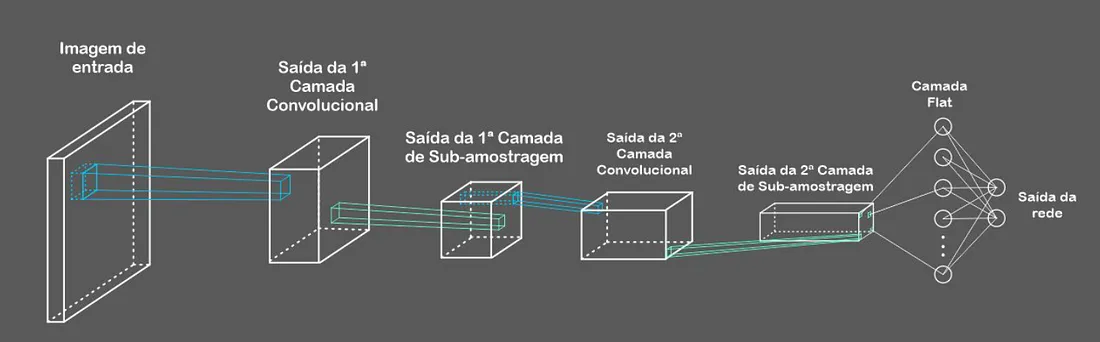
\includegraphics[width=1\linewidth]{cnn.png}
    \caption{Arquitetura de uma CNN.} \protect\href{https://vitorborbarodrigues.medium.com/conhecendo-a-vis%C3%A3o-do-computador-redes-neurais-convolucionais-e1c2b14bf426}{(\textcolor{blue}{Fonte})}
    \label{fig:cnn}
\end{figure}


\subsection{Componentes Técnicos}

\textbf{Fórmulas:}

\begin{equation}
(y * w)(i, j) = \sum_{m}\sum_{n} y(i+m, j+n) \cdot w(m, n)
\end{equation}

\begin{equation}
f(x) = \max(0, x)
\end{equation}

\begin{equation}
O = \left\lfloor \frac{n - f + 2p}{s} \right\rfloor + 1
\end{equation}

\begin{equation}
a^{[L]}_k = \frac{e^{z_k}}{\sum_{j=1}^{K} e^{z_j}}
\end{equation}

\subsection{Aplicação de CNN em Aplicativos de Namoro}

As Redes Neurais Convolucionais (CNNs) podem ser aplicadas eficazmente em aplicativos de namoro para entender e prever preferências visuais dos usuários, melhorando a experiência e personalização do serviço.

\begin{itemize}
    \item \textbf{Processamento de Dados de Imagem:}  
    Nos aplicativos de namoro, os usuários interagem com perfis, indicando suas preferências por meio de likes e dislikes. As CNNs podem ser treinadas para identificar padrões nas fotos dos perfis que recebem likes e dislikes, ajudando a determinar o que cada usuário considera atraente.

    \item \textbf{Treinamento da CNN:}  
    Um conjunto de dados grande e diversificado de imagens de perfis e interações de usuários é utilizado. A rede aprende a associar características visuais específicas com a probabilidade de um perfil receber um like.

    \item \textbf{Personalização de Recomendações:}  
    Uma vez treinada, a CNN pode ser integrada ao sistema de recomendação do aplicativo. Quando um novo perfil é apresentado, a CNN avalia as características visuais da imagem e prevê a probabilidade de um like com base nas preferências aprendidas.
\end{itemize}

Em resumo, a aplicação de CNNs em aplicativos de namoro é comum e muito eficaz como tecnologia de aprendizado profundo, potencializando o sucesso das interações e a eficácia de matches no aplicativo como um todo.


\section{Transformers}

\subsection{Introdução ao Conceito}
\textbf{}

\textbf{Definição:}  
Transformers são uma arquitetura de rede neural projetada para processar dados sequenciais de forma eficiente, utilizando o mecanismo de autoatenção. Introduzidos em 2017, os transformers superaram as redes recorrentes (RNNs) e as redes LSTM em diversas tarefas, especialmente no processamento de linguagem natural (NLP).

\textbf{Contextualização:}  
Transformers revolucionaram o campo do aprendizado profundo, particularmente em NLP, mas suas aplicações se expandiram rapidamente para outras áreas, incluindo visão computacional, processamento de áudio e aprendizado multi-modal. Sua capacidade de modelar dependências de longo alcance e capturar informações contextuais os tornaram o padrão ouro para a maioria das tarefas de NLP.

\subsection{Desenvolvimento Teórico}

\textbf{Explicação Detalhada:}

Os transformers são construídos com base em uma arquitetura de codificador-decodificador, que permite ao modelo analisar uma sequência de entrada, construir uma representação intermediária e, em seguida, gerar uma sequência de saída. Os principais componentes incluem:

\begin{itemize}
    \item \textbf{Mecanismo de Autoatenção:}  
    O mecanismo de autoatenção permite ao modelo pesar a importância de diferentes partes da sequência de entrada ao fazer previsões. Ele usa vetores de consulta, chave e valor para calcular scores de atenção, que determinam o foco em partes específicas da entrada.

    \begin{equation}
    \text{Attention}(Q, K, V) = \text{Softmax}\left(\frac{QK^T}{\sqrt{d_k}}\right)V
    \end{equation}

    Onde \(Q\), \(K\) e \(V\) são as matrizes de consulta, chave e valor, respectivamente, e \(d_k\) é a dimensão dos vetores de chave.

    \item \textbf{Codificadores e Decodificadores:}  
    O codificador transforma a entrada em uma representação de alto nível (vetor de contexto), enquanto o decodificador usa essa representação para gerar a saída.

    \item \textbf{Codificação Posicional:}  
    Como os transformers não possuem processamento sequencial inerente, eles utilizam codificações posicionais para injetar informações sobre a ordem dos tokens na sequência.

    \begin{equation}
    \text{PE}_{(pos, 2i)} = \sin\left(\frac{pos}{10000^{2i/d}}\right)
    \end{equation}
    \begin{equation}
    \text{PE}_{(pos, 2i+1)} = \cos\left(\frac{pos}{10000^{2i/d}}\right)
    \end{equation}

    Onde \(pos\) é a posição do token na sequência, \(i\) é o índice da dimensão, e \(d\) é a dimensão total dos embeddings.

    \item \textbf{Normalização de Camada e Conexões Residuais:}  
    A normalização de camada é usada para estabilizar e acelerar o treinamento. As conexões residuais ajudam na aprendizagem de redes profundas, mitigando problemas relacionados a gradientes desaparecendo.
\end{itemize}

\textbf{Fórmulas}

\begin{enumerate}
    \item \textbf{Autoatenção Escalonada:}  
    A autoatenção escalonada é calculada usando a seguinte fórmula, onde \(Q\), \(K\) e \(V\) representam as matrizes de consulta, chave e valor:

    \[
    \text{Attention}(Q, K, V) = \text{Softmax}\left(\frac{QK^T}{\sqrt{d_k}}\right)V
    \]

    Este mecanismo permite ao modelo identificar quais partes do texto são mais relevantes para cada parte da entrada.

    \item \textbf{Camadas de Normalização:}  
    A normalização de camada é aplicada para cada saída da camada, definindo a média e variância para estabilizar o treinamento:

    \[
    \text{LayerNorm}(x) = \frac{x - \mu}{\sqrt{\sigma^2 + \epsilon}}
    \]

    Onde \(\mu\) é a média e \(\sigma^2\) é a variância das ativações.
\end{enumerate}
\clearpage
  \begin{figure}
    \centering
    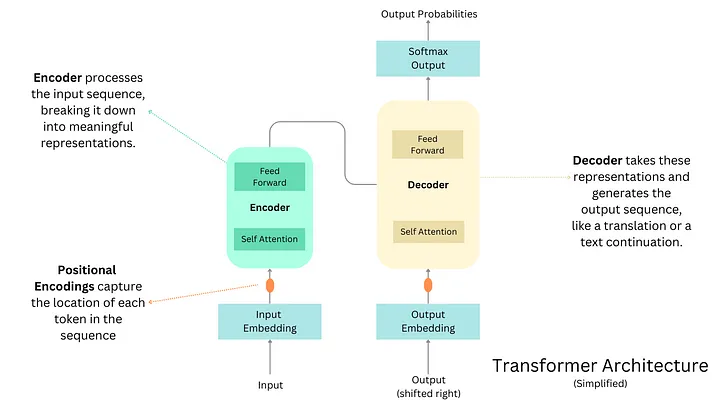
\includegraphics[width=0.8\linewidth]{transformer.png}
    \caption{Arquitetura de um Transformer.} \protect\href{https://medium.com/@tech-gumptions/transformer-architecture-simplified-3fb501d461c8}{(\textcolor{blue}{Fonte})}
    \label{fig:cnn}
\end{figure}
  \begin{figure}
    \centering
    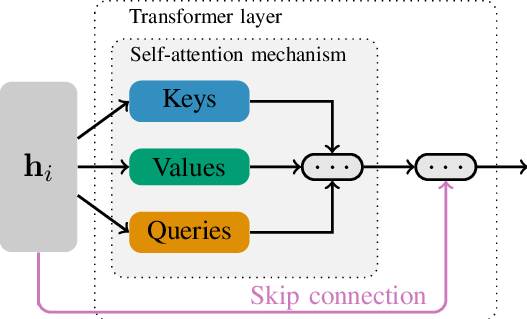
\includegraphics[width=0.4\linewidth]{selfattention.png}
    \caption{Mecanismo de Auto Atenção \cite{Vaswani2017}.}
    \label{fig:cnn}
\end{figure}



\subsection{Aplicação em Aplicativos de Namoro}

Transformers podem ser aplicados em aplicativos de namoro para aprimorar a análise de interesses e conexões sociais comuns entre usuários. Eles podem analisar descrições textuais, biografias de perfil e interações passadas para identificar interesses compartilhados e conexões sociais comuns, melhorando a qualidade das sugestões de matches.

\section{Redes Neurais de Grafos (GNNs)}

\subsection{Introdução ao Conceito}
\textbf{}

\textbf{Definição:}  
Redes Neurais de Grafos (GNNs) são uma classe de modelos de aprendizado profundo projetados para lidar com dados estruturados em grafos. Elas são capazes de capturar a topologia do grafo e aprender representações complexas de nós e arestas, aproveitando as relações intrínsecas e interações entre os componentes do grafo.

\textbf{Contextualização:}  
As GNNs têm sido amplamente adotadas em áreas como redes sociais, biologia computacional, sistemas de recomendação e processamento de linguagem natural, devido à sua capacidade de modelar dados não estruturados em um formato mais expressivo e relacional.

\subsection{Desenvolvimento Teórico}
\textbf{}

\textbf{Explicação Detalhada:}

As GNNs operam por meio da agregação de informações dos nós vizinhos, utilizando diferentes mecanismos de atualização e propagação de mensagens. Os principais componentes e operações incluem:

\begin{itemize}
    \item \textbf{Propagação de Mensagens:} 
    Este é o processo pelo qual cada nó coleta informações de seus vizinhos para atualizar sua própria representação. A propagação de mensagens permite que as GNNs capturem a estrutura local e as dependências de longo alcance no grafo.

    \begin{equation}
    \mathbf{h}_i^{(l+1)} = \text{AGGREGATE} \left(\left\{\mathbf{h}_j^{(l)}, \forall j \in \mathcal{N}(i)\right\}\right)
    \end{equation}

    \begin{equation}
    \mathbf{h}_i^{(l+1)} = \text{UPDATE} \left(\mathbf{h}_i^{(l)}, \mathbf{h}_i^{(l+1)}\right)
    \end{equation}

    Onde \(\mathcal{N}(i)\) representa o conjunto de vizinhos do nó \(i\), e as funções AGGREGATE e UPDATE são projetadas para combinar e atualizar as informações dos nós.

    \item \textbf{Normalização e Agregação:} 
    Métodos de normalização, como normalização simétrica, são usados para garantir que a contribuição de cada vizinho seja balanceada de acordo com o grau do nó. Isso promove uma propagação de informações mais consistente e robusta através do grafo.

    \item \textbf{Funções de Ativação e Pesos Treináveis:} 
    Funções de ativação, como ReLU, são aplicadas às representações agregadas, e pesos treináveis são usados para aprender as melhores transformações durante o processo de treinamento.
\end{itemize}

\clearpage
  \begin{figure}
    \centering
    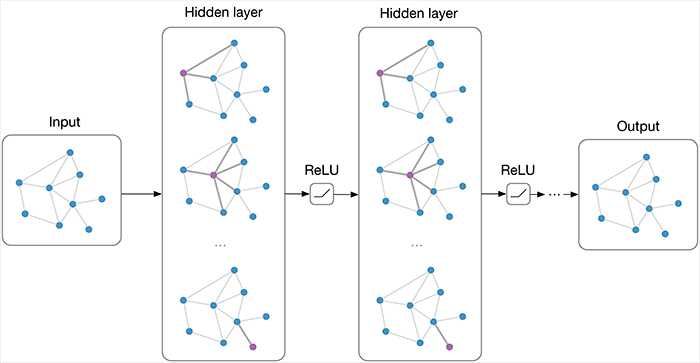
\includegraphics[width=0.8\linewidth]{image.png}
    \caption{Representação de uma GNN.} \protect\href{https://tkipf.github.io/graph-convolutional-networks/}{(\textcolor{blue}{Fonte})}
    \label{fig:cnn}
\end{figure}



\subsection{Componentes Técnicos}

\textbf{Fórmulas:}

1. \textbf{Propagação de Mensagens:}

\begin{equation}
\mathbf{h}_i^{(l+1)} = \sigma \left( \sum_{j \in \mathcal{N}(i)} \mathbf{W} \cdot \mathbf{h}_j^{(l)} + \mathbf{b} \right)
\end{equation}

Esta fórmula define a operação de uma camada em uma GNN, onde \(\mathbf{W}\) e \(\mathbf{b}\) são pesos treináveis, e \(\sigma\) é a função de ativação.

2. \textbf{Agregação com Normalização:}

\begin{equation}
\mathbf{h}_i^{(l+1)} = \sigma \left( \sum_{j \in \mathcal{N}(i)} \frac{1}{\sqrt{d_i d_j}} \mathbf{W} \cdot \mathbf{h}_j^{(l)} \right)
\end{equation}

Onde \(d_i\) e \(d_j\) são os graus dos nós \(i\) e \(j\), respectivamente.




\subsection{Conclusão}

As Redes Neurais de Grafos (GNNs) representam um avanço no aprendizado profundo, oferecendo um modo eficaz de modelar dados relacionais complexos. Em sistemas de recomendação para aplicativos de namoro, as GNNs podem ser utilizadas para explorar as interações e conexões sociais entre usuários. Ao modelar usuários e suas interações como nós e arestas, as GNNs conseguem identificar padrões de comportamento e compatibilidades baseadas não apenas em interesses comuns, mas também em influências sociais e interações passadas.

Essa abordagem pode aumentar a precisão das recomendações, ajudando a sugerir matches com maior potencial de sucesso e longevidade, oferecendo uma experiência de usuário mais personalizada e eficaz.
%
\section{Cafe: Predicting Physical Attraction with Deep Learning-Based Systems}

\subsection{Introdução ao Conceito}

\textbf{Definição:} \\
O projeto ``Cafe'' é um aplicativo de namoro que utiliza aprendizado profundo, especificamente redes neurais convolucionais (CNNs), para prever a atratividade física de indivíduos. Ele utiliza técnicas de aprendizado por transferência para personalizar a experiência do usuário, sendo uma referência valiosa para aplicar CNNs na análise de preferências visuais em trabalhos de conclusão de curso \textcolor{blue}{[\cite{DesiPilla}]}.

\textbf{Contextualização:} \\
No cenário atual dos aplicativos de namoro, a aparência física é frequentemente um fator decisivo. O ``Cafe'' visa otimizar esse processo através de algoritmos de deep learning, treinando modelos para analisar imagens de perfis de maneira eficiente e automatizada.

\subsection{Desenvolvimento Teórico}

\textbf{Explicação Detalhada:}

O projeto ``Cafe'' aplica técnicas de aprendizado por transferência, utilizando a arquitetura VGGNet como base para treinar redes neurais em um conjunto de imagens coletadas do Google. A CNN analisa imagens de perfis de namoro para prever se uma foto é atraente ou não, de acordo com as preferências do autor.



\textbf{Conjunto de Dados:} \\
As imagens usadas no treinamento foram retiradas do Google, abrangendo uma variedade de etnias e idades. Foram aplicadas técnicas de aumento de dados para melhorar a diversidade e representatividade do conjunto de dados.

\textbf{Modelagem de Preferências:} \\
A abordagem se concentra em personalizar recomendações com base em preferências pessoais, utilizando rótulos de ``gostar'' ou ``não gostar'' para treinar o modelo a prever a atratividade com precisão.
\clearpage
\begin{figure}
    \centering
    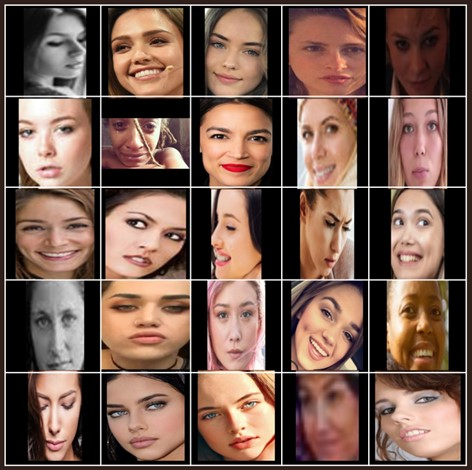
\includegraphics[width=0.8\linewidth]{faces.png}
    \caption{Exemplo de Imagens Usadas.} \protect\href{https://github.com/DesiPilla/cafe}{(\textcolor{blue}{Fonte})}
    \label{fig:cnn}
\end{figure}



\subsection{Componentes Técnicos}

\textbf{Adaptação do Algoritmo:}

\begin{itemize}
    \item \textbf{Camadas Densas:} As camadas densas finais do VGG16 são removidas e substituídas por novas camadas treináveis, otimizadas para classificar atratividade em perfis de namoro.
    \item \textbf{Transferência de Aprendizado:} A técnica de aprendizado por transferência é usada para economizar tempo computacional e melhorar a precisão, ajustando camadas pré-treinadas para o conjunto de dados específico.
\end{itemize}

\begin{itemize}
    \item \textbf{VGGNet e VGG16:} \\
    VGGNet é uma arquitetura de rede neural convolucional desenvolvida pelo Visual Geometry Group da Universidade de Oxford. Destaca-se por sua simplicidade e eficácia na classificação de imagens, utilizando camadas de convolução com filtros pequenos de 3x3, intercaladas com camadas de pooling. A VGG16 é uma variante que consiste em 16 camadas com parâmetros, incluindo 13 camadas de convolução e 3 camadas totalmente conectadas. Essa arquitetura é conhecida por sua profundidade e capacidade de aprender representações complexas de imagens \textcolor{blue}{[\cite{Simonyan2014}]}.

    \item \textbf{Aprendizado por Transferência:} \\
    O aprendizado por transferência é uma técnica que permite utilizar modelos previamente treinados, como o VGG16, para novas tarefas. Isso é feito ajustando as camadas finais do modelo para o novo conjunto de dados, economizando tempo e recursos computacionais ao aproveitar o conhecimento previamente adquirido pelo modelo \textcolor{blue}{[\cite{Krizhevsky2012}]}.

    \item \textbf{Explicabilidade (LRP):} \\
    O projeto também explora a explicabilidade dos modelos, utilizando técnicas como a Propagação de Relevância em Camadas (LRP). A LRP é uma técnica que ajuda a entender como as decisões são tomadas pela rede neural, identificando quais características de uma imagem são mais relevantes para as previsões do modelo. Isso é feito rastreando a contribuição de cada pixel na imagem original para a decisão final da rede, oferecendo uma visualização clara das áreas que mais influenciam as decisões do modelo \textcolor{blue}{[\cite{Bach2015}]}.
\end{itemize}

O ``Cafe'' demonstra o potencial de aplicar deep learning em aplicativos de namoro, otimizando o processo de recomendação com base em atratividade visual e preferências pessoais.

\section{Dataset OkCupid e Instagram Graph API}

\subsection{Utilização do Dataset OkCupid}

\textbf{Definição:} \\
O dataset OkCupid Profiles disponível no Kaggle é uma coleção rica de perfis de usuários da plataforma de encontros OkCupid. Ele inclui dados demográficos e preferências pessoais, como idade, gênero, localização, interesses e auto-descrições, tornando-o um recurso valioso para análises de comportamento e perfilagem de usuários \textcolor{blue}{[\cite{OkCupidProfiles}]}.

\textbf{Contextualização:} \\
Esses dados podem ser usados para implementar "Personality Aggregation" em sistemas de recomendação, identificando características comuns entre usuários e melhorando a personalização das recomendações. Por exemplo, informações textuais podem ser processadas usando técnicas de processamento de linguagem natural (NLP) para extrair insights sobre preferências pessoais e traços de personalidade.

\subsection{Integração com a API do Instagram Graph}

\textbf{Definição:} \\
A API do Instagram Graph é uma ferramenta que permite acessar dados de interações sociais e conexões entre usuários no Instagram. Com ela, é possível obter informações sobre quem um usuário segue, quem os segue, além de suas interações, como curtidas e comentários \textcolor{blue}{[\cite{InstagramGraphAPI}]}.

\textbf{Contextualização:} \\
Utilizando a API do Instagram Graph, pode-se modelar o grafo social de usuários, capturando as influências sociais que afetam as preferências de cada um. Este tipo de "Social Aggregation" é fundamental para compreender como as redes sociais influenciam comportamentos e escolhas, possibilitando recomendações mais precisas e baseadas em interações sociais reais.

\section{GraphRecWWW19}

\subsection{Introdução ao Conceito}

\textbf{Definição:}  
GraphRec é uma arquitetura de rede neural desenvolvida para recomendações sociais, utilizando redes neurais de grafos (GNNs). Essa abordagem integra informações de nós e a estrutura topológica de dados de grafo a alguns mecanismos presentes nos transformers, permitindo modelar de forma eficaz tanto as interações quanto as opiniões no grafo de usuário-item e no grafo social de usuário-usuário.\textcolor{blue}{[\cite{GraphRecWWW19}]}.
\textbf{Contextualização:}  
Em sistemas de recomendação social, os dados são frequentemente representados como grafos, onde nós representam usuários ou itens e as arestas representam interações ou relações sociais. GraphRec se destaca por sua capacidade de capturar e modelar essas relações complexas, combinando informações de diferentes tipos de grafos para melhorar a precisão das recomendações.

\subsection{Desenvolvimento Teórico}

\textbf{Explicação Detalhada:}

GraphRec utiliza uma combinação de técnicas de Graph Neural Networks (GNNs) e atenção para modelar dois tipos principais de grafos: o grafo usuário-item e o grafo social usuário-usuário. Esses componentes trabalham em conjunto para melhorar a capacidade do sistema de recomendação ao integrar múltiplas fontes de informação.

\begin{itemize}
    \item \textbf{Grafo Usuário-Item:}  
    Neste grafo, as arestas representam interações entre usuários e itens, muitas vezes acompanhadas de opiniões ou avaliações. O modelo utiliza agregações de itens para capturar preferências dos usuários com base nas interações passadas.

    \item \textbf{Grafo Social Usuário-Usuário:}  
    Este grafo modela as relações sociais entre usuários. A agregação social permite que o modelo entenda a influência social e como as relações entre usuários podem impactar suas preferências.

    \item \textbf{Integração com Mecanismo de Atenção:}  
    GraphRec aplica mecanismos de atenção para dar pesos diferentes a diferentes conexões no grafo, permitindo uma modelagem mais precisa das relações complexas entre nós.
\end{itemize}

\clearpage
\begin{figure}
    \centering
    \vspace{-2cm}
    \hspace*{-2.5cm} % Ajuste o valor em centímetros conforme necessário
    \includegraphics[width=1.3\linewidth]{modelo.png}
    \caption{Modelo do GraphRechWWW19} \protect\href{https://github.com/wenqifan03/GraphRec-WWW19}{(\textcolor{blue}{Fonte})}
    \label{fig:cnn}
\end{figure}

\subsection{Componentes Técnicos}

\textbf{Adaptação do Algoritmo:}

\begin{itemize}
    \item \textbf{Item Aggregation to Personality Aggregation:}  
    Nesta adaptação, o componente de agregação de itens pode ser alterado para agregar traços de personalidade, considerando traços de personalidade como itens para identificar preferências comuns entre usuários.

    \item \textbf{Social Aggregation:}  
    Este componente permanece inalterado, continuando a capturar influências sociais baseadas nas conexões entre usuários no grafo social.

    \item \textbf{Adição de Visual Aggregation:}  
    Um novo componente de agregação visual pode ser introduzido, onde Redes Neurais Convolucionais (CNNs) são usadas para extrair características visuais das imagens dos usuários, analisando aquelas que recebem likes e dislikes.
\end{itemize}

Com essas adaptações, GraphRec pode ser ajustado para analisar não apenas preferências de item, mas também traços de personalidade e preferências visuais, tornando o sistema de recomendação mais abrangente e personalizado para aplicativos de namoro.



%
\input{tex/5_Conclusao}%

%\apendice{Apendice_Fichamento}{Fichamento de Artigo Científico}%
%\anexo{Anexo1}{Documentação Original \unbcic\ (parcial)}%

\bibliographystyle{apalike}
\bibliography{bibliografia}%

\end{document}%
